% !TEX root = ../main.tex
\begin{tikzpicture}[remember picture,overlay]
    \node[anchor=north, yshift=0.10cm] at (current page.north) {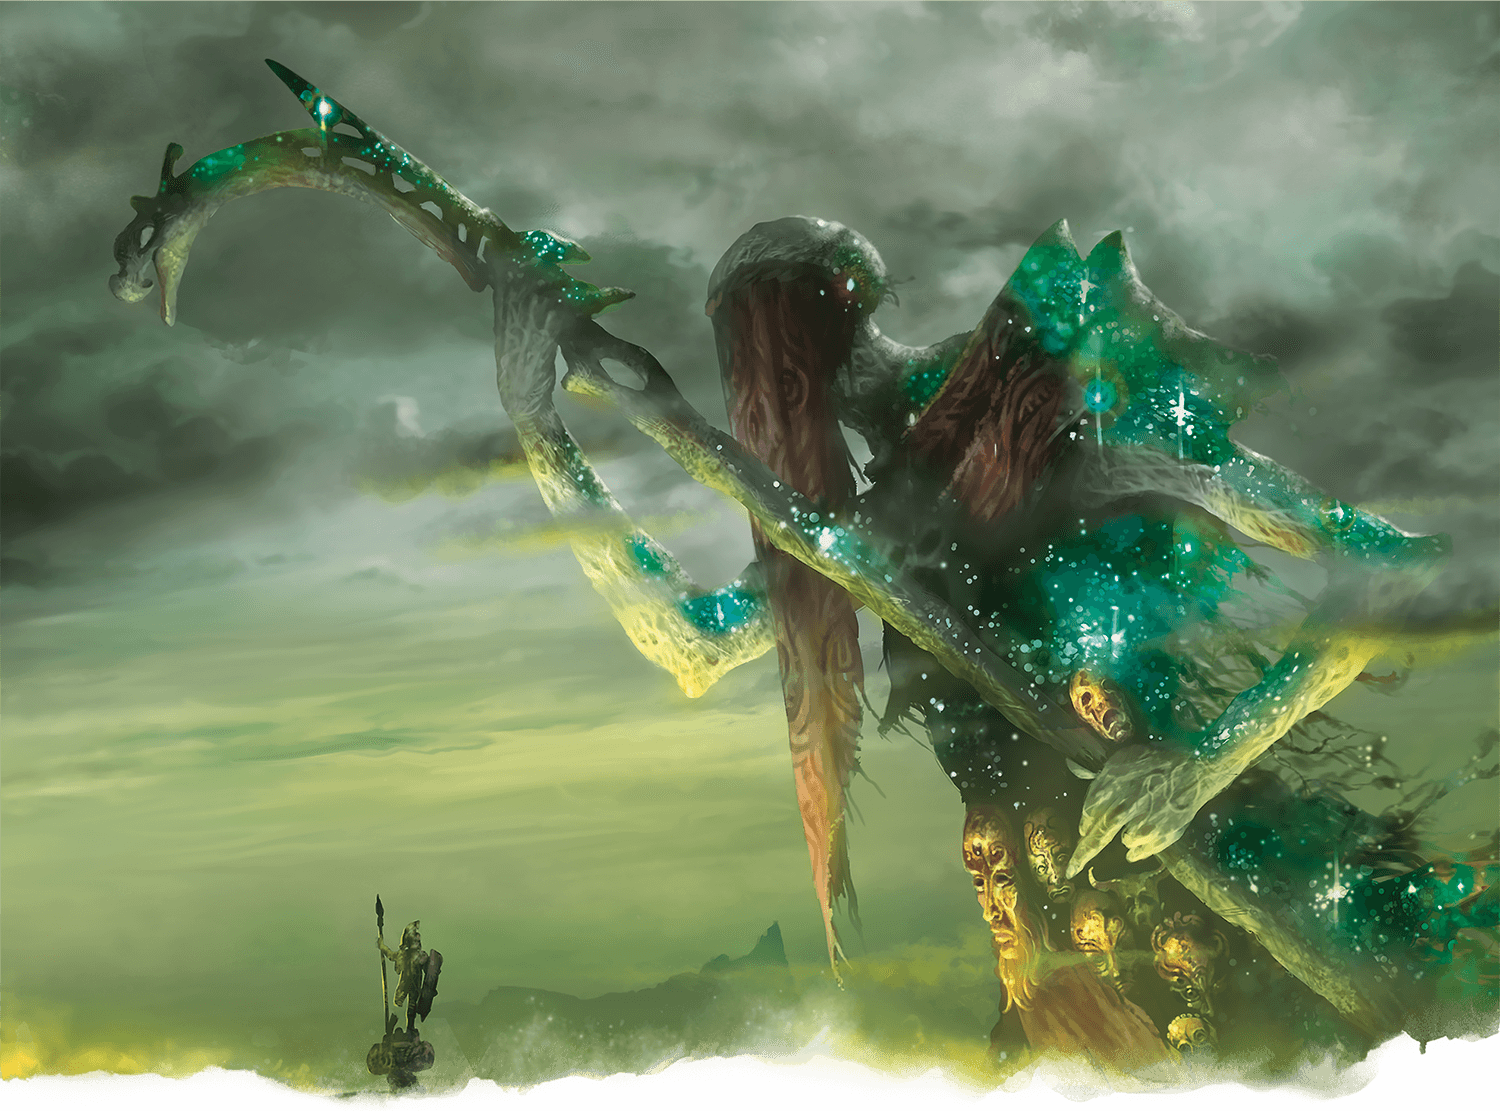
\includegraphics[width=\pdfpagewidth]{02viphoger/img/10athreos.png}};
\end{tikzpicture}

\vspace{14.0cm}

\section{Therism} \label{ssec::therism}

A pantheon of fifteen gods guides religious life on Viphoger.
From the sun and agriculture to death and passage into Nyx, the gods oversee the forces of nature and the most important aspects of mortal life.
These gods are quite real to the people of Viphoger, who see them moving across the sky at night and sometimes encounter them face to face.
Thus, most people perform rituals and devotions that honor various gods, hoping to win their favor and stave off their wrath.
They tell and retell the stories of the gods' deeds --- even as they watch those stories continue to play out in the vastness of the night sky.

Therism is the main religion practiced in Viphoger.
While both religions draw from the same pantheon, Tanethism and Therism couldn't have less in common.
The former was designed by a scholar and forced on their by a king, while the latter developed gradually from the gat settlers of the Sylvan Canyon.

\pagebreak~
\vspace{14.5cm}

In their new land, they saw the gods' visage in the sky, equatting them to their ancient deities.
Not every mortal serves or acknowledges the gods, though.
Some philosophers in the schools of Mephetis teach that the gods of the pantheon are subordinate to a higher reality, perhaps the sky itself.
And other people, particularly leonin, believe that the gods are undeserving of mortal reverence.

\subsubsection{Worship}
    The most prevalent form of expressing reverence is the practice of libation, pouring out a splash of wine or water in honor of the gods.
    Pious people perform a simple rite of prayer and libation every morning and evening at a household altar or hearth, while the less devoted might still pour out a splash of wine before drinking the rest.

    The defining feature of a Theran temple is a statue of a god.
    Worshipers kneel before it, touch and kiss it, drape it in garlands and fine cloth, and leave offerings before it.
    % These acts are sometimes spontaneous outpourings of love or gratitude, and sometimes petitions, imploring the god to cure an illness, send rain for crops, guarantee a safe journey, or perform any other favor related to the god's sphere of influence.

    % Most people aren't devoted to a single god, though many prefer some gods over others. Someone might ask Pharika to spare a loved one from disease, then later offer prayers to Karametra for a bountiful harvest or to Thassa for safety on a sea journey.

    % Considering their significance to the people of Viphoger, this section includes a list of the 15 gods of the Therist pantheon, including a short description of each.

\pagebreak

% !TEX root = ../main.tex
\subsection*{Athreos, God of Passage} \label{ssec::athreos}
    \subparagraph{Tides} Indigo, Silver.

    All mortals are destined to face Athreos, the River Guide, when their lives come to an end.
    The god of passage ferries the dead across the Tartyx River, conveying each mortal soul to its destiny in Nyx.
    For most people, Athreos embodies the greatest mysteries of existence --- the terror and wonder of life's last moment and the revelation of one's ultimate fate in the afterlife.
    % Athreos is no judge, though.
    The veiled, silent god undergoes no deliberations and makes no exceptions.
    The River Guide reads the truth of each soul and bears it unfailingly to its proper place in Nyx.
    There is no haggling and no sympathy on Athreos's skiff, the god having heard and denied every mortal plea.

    Athreos appears as a gaunt figure cloaked in ragged robes and a collection of golden masks.
    What little can be seen of their body is unsettling, its gray flesh stretched thin over a barely et skeleton.
    The River Guide is never without their ancient staff, Katabasis, which they transforms into the ferryboat they use to ply the Rivers That Ring the World.
    Athreos can change shape but rarely, if ever, takes on other forms.

    % \begin{figure}[t]
    %     \centering
    %     
\includegraphics[width=0.47\textwidth]{02viphoger/img/10s_athreos.png}
    % \end{figure}

    \subsubsection{Worshiping Athreos}
        Most funeral traditions include small offerings and words of reverence to Athreos.
        Predominant among these traditions is burying or burning the dead with a clay funerary mask, to ``frame'' the identity of the dead for Athreos, and with at least one coin, so a soul might pay Athreos to ferry them to Nyx.
        % Some people are laid to rest with large amounts of grave goods.
        Memorial practices vary widely by culture, from tearful, somber affairs to lively celebrations.
        These rituals serve more as catharsis for the living than as meaningful boons to Athreos, though.
        The River Guide cares only for the single coin they're owed by any who board their skiff.

        During the feast of Necrologion, pious souls silently spend the day reading ancient memoirs or writing messages for their own descendants.
\subsection*{Ephara, God of the Polis} \label{ssec::ephara}
    \subparagraph{Domains} Indigo, Blue.

    As god of the polis, Ephara sees themself as the founder of civilization.
    They watch over cities, protecting them from outside threats.
    They are credited with establishing the first code of law, which Mephetis has preserved and the other poleis have imitated.
    Even more important, they help cities reach their highest potential, becoming centers of scholarship, industry, and art.

    Ephara appears as a huge animated statue wearing a stone crown, resembling the capital of a column.
    When they choose to walk about their cities at a mortal's scale, they often take on the form of a gat.
    In either form, they are always dressed in blue and white, and their expression is usually serious, but not unkind.
    They often carry a large urn on one shoulder, with the dark, star-studded sky pouring from it and dissolving into mist as it hits the ground.

    % \begin{figure}[b]
    %     \centering
    %     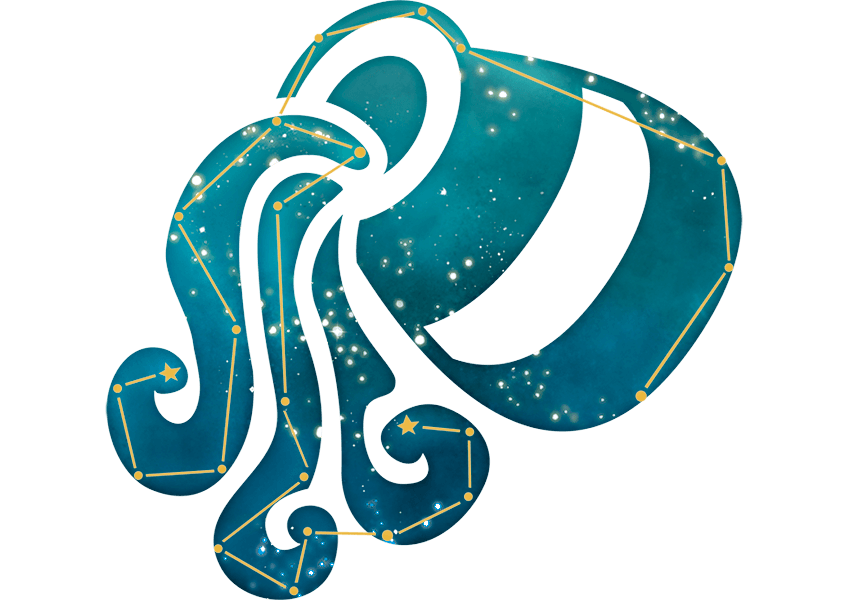
\includegraphics[width=0.47\textwidth]{02viphoger/img/10s_ephara.png}
    % \end{figure}

    \subsubsection{Worshiping Ephara}
        To an extent, Ephara's devout show their faith by going about their lives and contributing to society.
        Midday services at Ephara's temples often feature a brief prayer, followed by a longer talk from an industrial or civic leader on a topic of general interest.
        Attendants often bring meals to eat while on a break from their jobs.

        Ephara's face is a common sight in cities.
        Marble buildings, stone walls, and similar surfaces usually feature a sculpture or relief of their visage.
        People often swear oaths or engage in verbal disputes in front of these images, believing they won't let a falsehood told in front of them go unpunished.
        Whether they actually intervenes is unclear, but conflicts that play out this way are often resolved peacefully, without a need for the justice system to get involved.

\subsection*{Erebos, God of the Dead} \label{ssec::erebos}
    \subparagraph{Domains} Silver.

    Erebos is the god of death and Nyx, lord of all that has ever lived.
    % They preside over the bitterness, envy, and eventual acceptance of those who suffer misfortune.
    Their hoarding of both souls and the treasures the dead carry into Nyx see them worshiped by those who desire to collect and keep wealth.

    Erebos's very presence is stifling, and those who come face to face with them often depart in despair.
    They are jealous and tyrannical within their realm, but unlike their brother Heliod, they neither bluster nor try to expand their influence.
    They wait patiently, secure in the knowledge that everything belongs to then in the end.

    Erebos most frequently appears as a slender, gray-skinned gat with two large, outward-curving horns, wielding a long black whip.
    They also appear in the form of a black asp, a cloud of choking smoke, or an animated golden idol.

    % \begin{figure}[b]
    %     \centering
    %     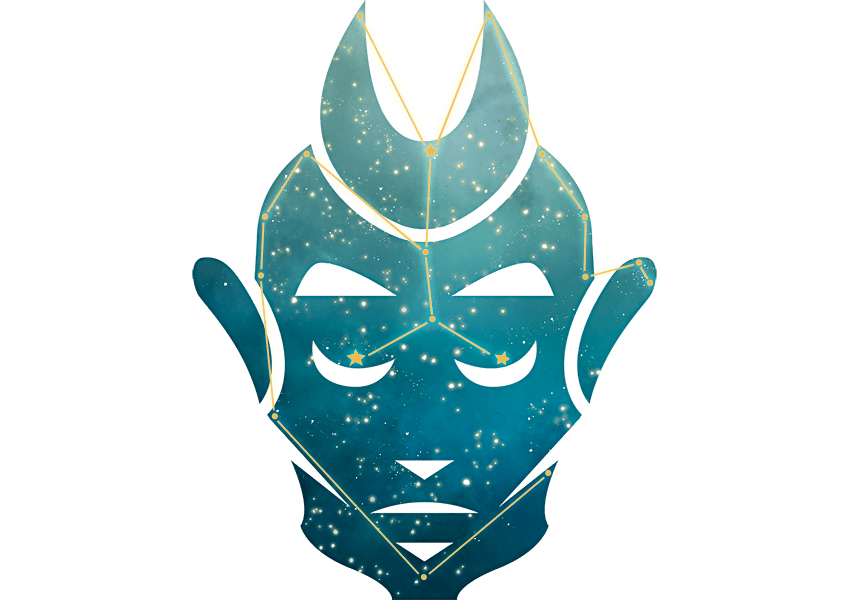
\includegraphics[width=0.47\textwidth]{02viphoger/img/10s_erebos.png}
    % \end{figure}

    \subsubsection{Worshiping Erebos}
        To many mortals, Erebos is primarily concerned not with death, but with gold.
        Most of their followers downplay their association with death and misfortune, praying to them for material wealth.
        Others pray to them because they want to be more accepting of their misfortune.
        These individuals see themselves as beyond hope, asking only that Erebos grant them the strength to endure until they enter their realm at their predestined time.

        A smaller but more dangerous group of Erebos worshipers are those who glorify death.
        These cultists and assassins congregate in secret in communities across Viphoger, engaging in campaigns of violence.

        The only major festival dedicated to Erebos is the Katabasion or ``the Descent'', features a ceremony in which worshipers make a symbolic journey into Nyx.
        The supplicants enter a cave, offer prayers and sacrifices to Erebos in utter darkness, and slowly make their way back to the surface just before sunrise.

% !TEX root = ../main.tex
\subsection*{Heliod, God of the Sun} \label{ssec::heliod}
    \subparagraph{Domains} Light.

    Heliod is the radiant god of the sun.
    According to myth, they ensure that the sun rises every day to provide light and warmth to the world.
    Every inhabitant of Viphoger acknowledges their dominant presence, and nearly everyone at least pays lip service to the idea of giving them worship and honor.

    Pride and self-assurance radiate from Heliod as light floods from the sun.
    They are cheerful and sociable, enjoying the company of others and forming bonds easily.
    Their friendship can be as easily lost, though, turning them from ally to enemy as the consequence of a single misstep or perceived betrayal.

    Heliod has appeared to mortals in a variety of forms, but they prefers the appearance of a sun-bronzed gat in their forties, dressed in a flowing tunic of golden cloth.
    Their profile is noble, highlighted by a strong chin and a short beard, and they boast the broad chest of a perfectly fit athlete.
    Their hair is glossy black, and their head is crowned with a golden wreath.
    They are also fond of appearing as a brilliant white horse or a radiant golden stag.
    In any guise, they look lit by the sun, even when they travel across the night sky.

    \subsubsection{Worshiping Heliod}
        The brilliance of Heliod's sun is impossible to ignore.
        Thus, virtually everyone on Viphoger pays at least grudging respect to the sun god in forms of worship that range from simple gestures to days-long celebrations.

        Some families, particularly in the polis of Mephetis, follow a practice of bowing in the direction of dawn's first light --- or winking, in a gesture of respect for the sun god's luminous ``eye''.
        More dedicated worshipers offer short litanies at dawn, noon, and dusk, acknowledging the sun's passage across the sky.

\subsection*{Iroas, God of Victory} \label{ssec::iroas}
    \subparagraph{Domains} War.

    Iroas is the steadfast god of honor and victory in war.
    When soldiers march to battle, their voice is the thunder of their footsteps and the crash of spear on shield.
    Soldiers, mercenaries, and athletes all pray for Iroas's favor in securing victory.
    Common folk pray to Iroas for courage and fortitude in times of struggle, for their is the battle nobly fought and won.

    Bold and confident with a soldier's demeanor, Iroas is the pinnacle of martial pride and bearing.
    They are stoic almost to a fault, but also exhibits a wry sense of humor.
    Those who honorably shed blood in Iroas's name can count on their support.
    Cowards and oath breakers are to be despised, and traitors don't deserve mercy in battle.

    Iroas most often appears as a powerfully built gat with a bull-like body, clad in gleaming armor and wielding a spear and shield.
    They speak in a booming baritone that projects power, confidence, and courage.
    They have been known to appear as a burly soldier or a mighty bull before their followers.
    Whatever form they choose, Iroas carries themself with precision and majesty at all times and doesn't tolerate disrespect or undue informality from those who would deal with them.

    \subsubsection{Worshiping Iroas}
        Iroas is interested not in pretty words, but in great deeds.
        The faithful of Iroas show their piety by comporting themselves well in contests of athleticism or skill.
        Swearing an oath to win a battle in Iroas's name and failing to do so is a great shame upon a warrior, thus such a promise is never uttered lightly.

        The fifth month of the Fagalian calendar is Skenion, named for an annual commemoration of the Mephetian conquest of Natumas.
        This victory cemented Mephetis's control over the entire peninsula.
        But in Akhosh, the month is called Iroagonion, for the Iroan Games.
        These games are the grandest display to honor Iroas.
        To even compete in the Iroan Games is considered noteworthy, as the poleis send only their finest athletes.
        The grand prize, besides a ceremonial wreath, is the opportunity to be visited by Iroas themself.

\subsection*{Karametra, God of Harvests} \label{ssec::karametra}
    \subparagraph{Domains} Life, Nature.

    Karametra is recognized as the serene, maternal god of the harvest, her arms spread wide as she offers bounty to her worshipers or cradles communities in her embrace.
    Almost every uman settlement contains at least a modest shrine to solicit her favor, and she is closely associated with Setesh, the center of her worship.

    Wise and even-tempered, Karametra values community, stability, and the balance of nature.
    She is the god of maternity, family, orphans, domestication, and agriculture, as well as defense of the home and territory.

    Karametra appears to mortals as a motherly figure with hair made of ordered rows of leaves that shroud her eyes from view.
    She is always shown in art (and often seen in the night sky) seated on her throne, which is formed from a tangle of grape vines growing out of a collection of jugs and amphorae that surround her.
    An elaborately carved wooden canopy extends above her, and a giant sable --- her faithful companion --- curls around the base of the throne at her feet.
    In one hand, she holds a harvester's scythe.

    \subsubsection{Worshiping Karametra}
        The earth's fertility is essential for mortal life to continue.
        Those who live in the modern poleis might not be as aware of that fact as those who farm their own food, but even they long for children, know the pinch of hunger, and feel the turn of the seasons.

        Prayers to Karametra focus on asserting Karametra's constancy and bounty, praising the god's love and generosity.
        Worshipers of Karametra gather for a feast once a month, on the evening of the full Fagal, that celebrates the god's role in parenthood and community.
        New parents receive gifts and blessings, and young couples sneak away into the woods in hopes of finding sweet berries and sweeter kisses.

% !TEX root = ../main.tex
\subsection*{Keranos, God of Storms} \label{ssec::keranos}
    \subparagraph{Domains} Knowledge, Tempest.

    Keranos is the god of storms and wisdom.
    Merciless and impatient, Keranos is equally likely to strike out at mortals with a bolt of inspiration or a blast of lightning.
    To revere Keranos is to exult in the power of wisdom, clarity of purpose, and the fury of the storm.
    They are favored by tinkerers, inventors, and sailors as well as those seeking solutions to intractable problems.
    They don't tolerate the company (or the worship) of fools, and they despise vapidity and indecision.

    Keranos rarely appears directly to mortals, preferring to communicate through an epiphany or a crashing bolt of lightning.
    When they do deign to manifest in the mortal world, Keranos prefers the form of a stout, bearded, gat wearing a purple loincloth girdled in a steel chain belt with a clasp in the form of a wyvern's skull.
    Their bearing is upright and stern, with a clipped, brusque way of speaking.
    Particularly clever plans and observations bring a hint of a smile to their face.
    When interacting with mortals, Keranos sometimes appears in the form of a great horned owl with lightning strikes flashing in its eyes.

    \subsubsection{Worshiping Keranos}
        Keranos's name is often invoked by those amid a storm who seek safety, or by someone who is faced with a particularly difficult problem.
        Only the foolhardy call out to Keranos frivolously or in jest, since they might well smite the offender with a bolt from the blue.

        In Akhosh, where Prince Cymede actively promoted the worship of Keranos, elaborate ceremonies are conducted beginning just before the first summer thunderstorm.
        Intricate, open-framed sand paintings with complex geometric shapes are created by dancers in flowing blue silken wraps.
        Then, as the rains fall, the paintings are washed away, symbolizing the impermanence of genius and the power of change.
        Akhoash oracles strive to predict the exact time of the first storm in hopes of allowing enough time to stage the celebration.
        A similar festival in Mephetis, called the Astrapion (``Lightning Festival''), happens during the third month of the year.

        On the last day of every month, Keranos's priests and laity bring offerings of fish and distilled spirits to their temples.
        The fish are cooked under a skylight open to the stars, with a shot of spirits thrown on the fire.

\subsection*{Klothys, God of Destiny} \label{ssec::klothys}
    \subparagraph{Domains} Knowledge, War.

    Believed to have sprung into existence during Yuadrem's earliest days, Klothys is the god of destiny and, along with Kruphix, one of the world's original deities.
    They oversee the order of the cosmos, ensuring that all things remain in their proper place, knowing how easily the cosmic balance could be undone if they were not vigilant.
    On the heels of a near-catastrophic upset of the cosmic order --- the rise to godhood and subsequent defeat of the gat Xenagos --- Klothys has emerged from the Underworld for the first time in mortal memory to untangle the strands of destiny and set the world right.

    Klothys typically appears as a gat with six curling horns and an impossibly long mane of pale hair that cascades around their horns, drapes over their eyes, and spools into their spear-like weapon and the various other spindles they carry.

    Beneath their outward calm, Klothys seethes at the way mortals and gods alike have pulled apart and rearranged the threads of destiny to feed their petty ambitions.
    Their peaceful mien falls away in the presence of such villains.
    In their rage, their red-glowing eyes come into view through the veil of their hair, and they wield burning strands of hair as a devastating weapon.

    \subsubsection{Worshiping Klothys}
        Klothys doesn't trace their origins to mortal devotion, and they have languished in obscurity for almost the whole of Viphoger's history.
        They don't need worship to sustain or empower them, and they don't seek out reverence or demand it.
        By and large, mortals are irrelevant to them, except insofar as they have played a role in tangling the strands of destiny by defying nature's order.

\subsection*{Kruphix, God of Horizons} \label{ssec::kruphix}
    \subparagraph{Domains} Knowledge, Trickery.

    Kruphix is the enigmatic god of mysteries, horizons, and the passage of time.
    Their followers claim that they know not only everything that is known at present, but everything that has ever been known by anyone.

    Quiet surrounds Kruphix like a shroud.
    Standing apart from the other gods, they speak rarely, even to their most favored followers.
    When they do communicate, it is often as a barely audible whisper.
    Kruphix can speak with a booming voice directly into the minds of all the other gods simultaneously, though, doing so when something threatens the cosmic order.

    Kruphix's true form is more abstract than that of any of the other gods.
    They appear only in star-filled silhouette, usually as a hooded, four-armed figure of indeterminate species and gender.
    Two of the stars in their ``body'' often shine brightly, suggesting eyes.
    Kruphix's starry silhouette sometimes takes the form of a bird or a whale.

    \subsubsection{Worshiping Kruphix}
        Many pray to Kruphix when they need to find something lost, but few dedicate themselves to their worship.
        Cults devoted to Kruphix fiercely guard their secrets, and their initiates refrain from drawing attention to themselves.
        Some followers and champions of Kruphix travel the world in secret, searching for hidden truths.
        Many use secret signals to enable them to find safe lodging with other worshipers nearly anywhere.

        Rituals honoring Kruphix are usually performed at boundaries, both temporal and spatial: shorelines, riverbanks, equinoxes, and sunsets.
        One of the god's greatest festivals is the Agrypnion (``The Watching''), which marks the end of summer and the close of the year.

% !TEX root = ../main.tex
\begin{tikzpicture}[remember picture,overlay]
    \node[anchor=north, yshift=0.10cm] at (current page.north) {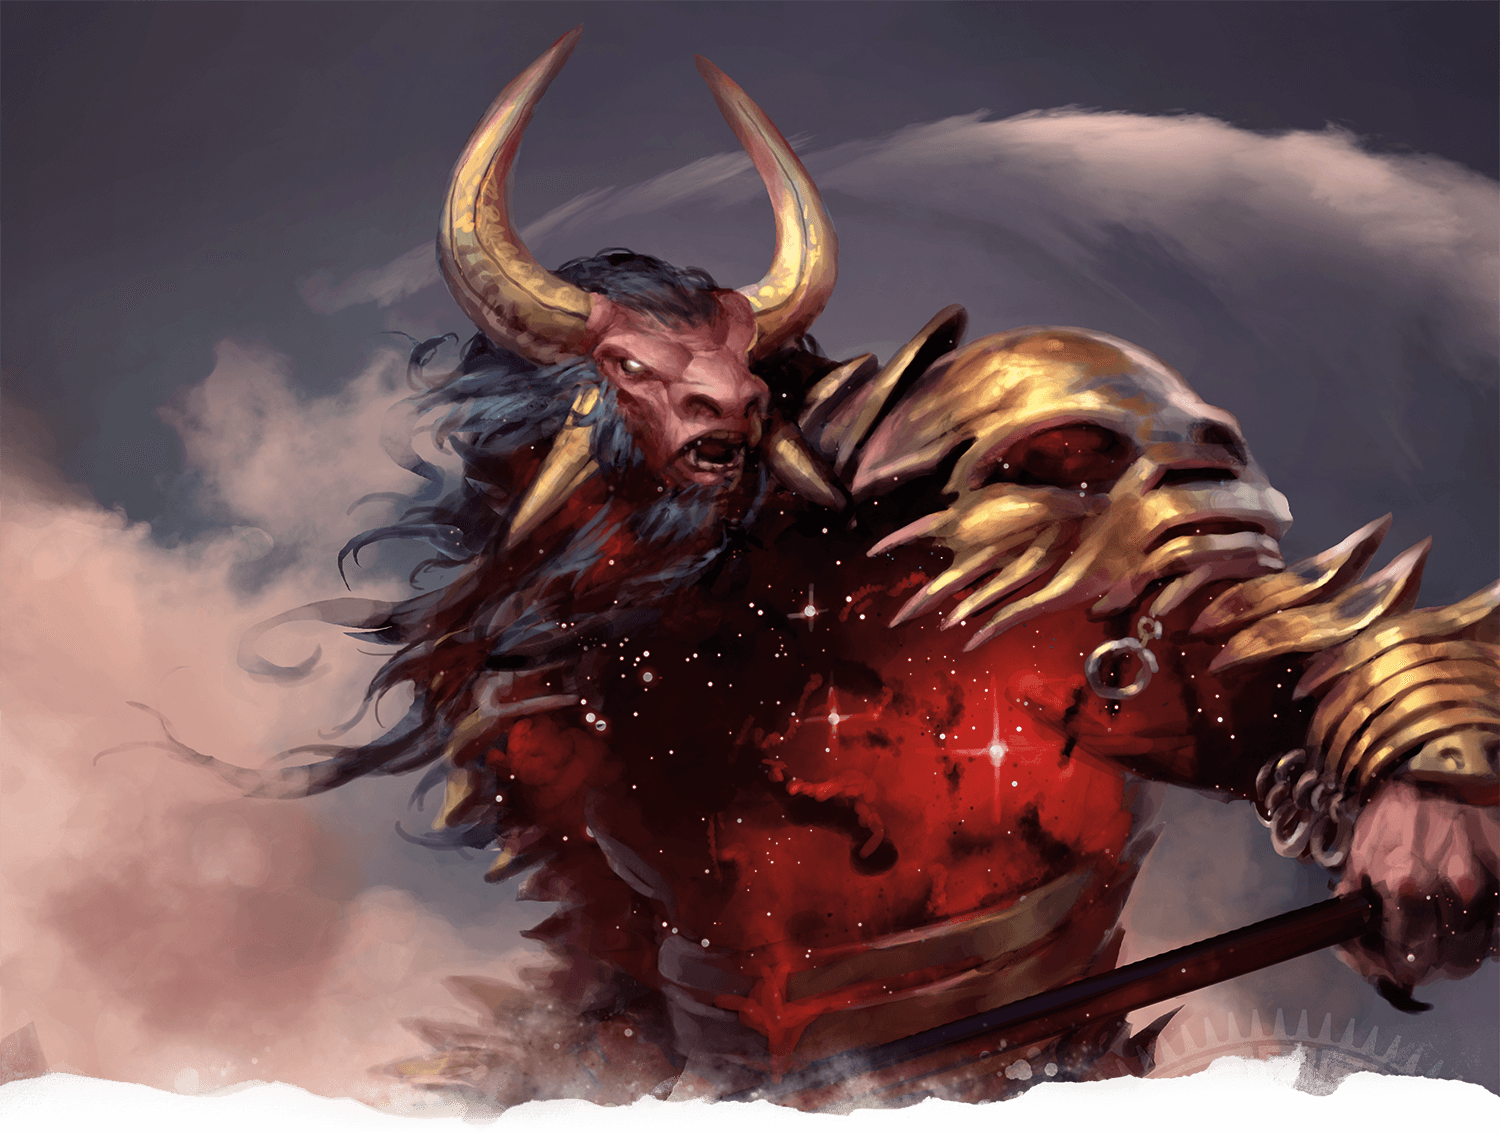
\includegraphics[width=\pdfpagewidth]{02viphoger/img/10mogis.png}};
\end{tikzpicture}

\vspace{13.5cm}

\subsection*{Mogis, God of Slaughter} \label{ssec::mogis}
    \subparagraph{Domains} War.

    Mogis is the god of slaughter, violence, and war.
    They are hatred unrestrained, empathy denied, and mercy forgotten, an entity whose very presence incites mortals to violence.
    Soldiers fear succumbing to their blood lust lest they dishonor themselves, but the vengeful and forsaken call to Mogis for the gift of their rage.
    They are the sibling of Iroas, god of victory, and their antithesis in matters of warfare.

    % The anger and malice radiating from Mogis is almost palpable.
    % They exercise no control over their temper or their urges and lash out at subordinates at the slightest provocation.
    % Akhoash soldiers are warned that to give in to their seductive battle rage is to risk becoming an androphage --- a bloodthirsty killer wholly consumed by Mogis's fury.

    Mogis cuts a terrifying figure, appearing as a four-horned treb gat of incredible size clad in spiked bronze armor and wielding a massive ebon greataxe.
    They don't debase themself by appearing in other guises to mortals --- to behold them is to behold the cruelty of war personified.
    They hunger endlessly to defeat their brother Iroas in combat and thus become the sole avatar of war among mortals.

    \begin{figure}[b]
        \centering
        
\includegraphics[width=0.47\textwidth]{02viphoger/img/10s_mogis.png}
    \end{figure}

    \pagebreak~
    \vspace{14.0cm}

    \subsubsection{Worshiping Mogis}
        Mogis exhorts their followers to channel their hatred and rage into ever greater acts of cruelty and violence.
        They demand actions over words, making their followers a dangerous lot.
        From the spurned lover thirsting for revenge to the blood-drenched warrior on the battlefield, all honor Mogis with the shedding of blood in anger.

        % Treb gats are the most ardent worshipers of Mogis and regularly hold bloody rites in their honor.
        % Warchanters, the clergy of Mogis, whip their marauders into a near-mindless frenzy before battle; the ensuing slaughter gives glory to Mogis's name.

        % The appearance of a blood moon is a most holy occasion for the faithful of Mogis, since the moon represents their hateful crimson eye.
        % At such times, their followers prepare and consume a feast of meat, either raw or barely cooked, along with copious amounts of intoxicants, followed by ritual self-mutilation --- scarring themselves to demonstrate their devotion to Mogis.

\subsection*{Nylea, God of the Hunt} \label{ssec::nylea}
    \subparagraph{Domains} Nature.

    Nylea is the wild, carefree god of the hunt.
    They claim dominion over the whole of the natural world, particularly hunger and predation, the seasons, metamorphosis and rebirth, and the forest.

    Nylea is among the most gregarious of the gods, and can be spotted frolicking joyfully with their Nyxborn lynx, Halma, or their favorite nymph, Theophilia.
    But they also savor solitude, and on the hunt they are deadly serious, almost animalistic, in their mood.
    They are nearly as quick to anger as their sibling Purphoros, enacting swift revenge on those who harm the natural realm.

    Nylea usually appears as a green-skinned dryad with woody extremities.
    Their hair is made of vines and leaves that change with the seasons.
    They might also appear as a majestic specimen of any animal, most frequently a lynx or a wolf.
    When they desire stealth or solitude, they might take the form of a tree, usually an oak or an olive.

    \begin{figure}[b]
        \centering
        
\includegraphics[width=0.47\textwidth]{02viphoger/img/10s_nylea.png}
    \end{figure}

    \subsubsection{Worshiping Nylea}
        Mortals all over Viphoger pray to Nylea when they rely on hunting or nature's whims for their livelihood.
        Their most ardent followers are bughna gats and humans (particularly those who live in Setesh and in the wilds), and nymphs of all kinds, especially dryads.
        Few leonin worship any of the gods, but of those who do, many favor Nylea with their prayers.

        Nylea blesses those who are kind to animals, considering such acts as wordless prayers.
        Those who must kill a dangerous natural animal or cut down trees often pray to Nylea for forgiveness, sometimes leaving food for other animals or planting new trees as atonement.

\pagebreak

\subsection*{Pharika, God of Affliction} \label{ssec::pharika}
    \subparagraph{Domains} Death, Knowledge, Life.

    Pharika is a god of affliction and medicine, alchemy and aging.
    % In the earliest days of the Sylvan Canyon, Pharika seeded the world with countless secret truths --- mysteries of medicine, minerals with strange properties, nexuses of magic, and the like --- which they hid among Nylea's wilds and the shadows of Erebos's Nyx, leaving clues where mortals might find them.
    It isn't altruism that drives them; they study the innovation and suffering of mortals, deciphering in them ever greater mysteries as they treat Viphoger as their personal laboratory.

    Pharika typically takes the form of a qulbaba ird with the lower body of a snake, similar to a couatl.
    Their body is thickly scaled and a pair of bronze-scaled vipers seamlessly emerge from their chest.
    They are never without their kylix, a drinking cup within which they can produce virtually any medicine or toxin.
    When their aims require subtlety, Pharika often takes the form of a serpent, or sometimes an aged gat.

    % Little escapes Pharika's cool gaze.
    % Even when outwardly friendly, they are cunning and calculating, watching for the slightest sign of weakness or desire that they can exploit later.
    % Those who offend them rarely recognize their misstep until they strike.

    \begin{figure}[t]
        \centering
        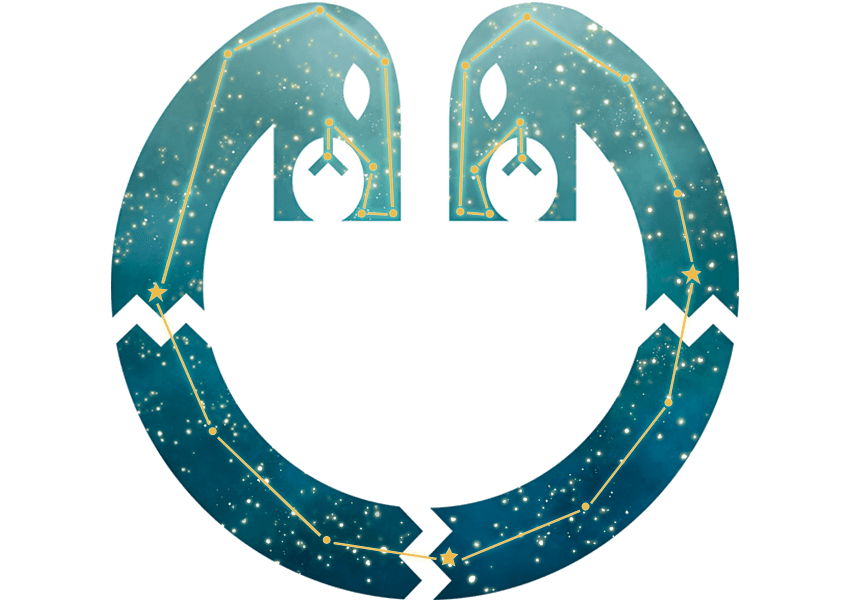
\includegraphics[width=0.47\textwidth]{02viphoger/img/10s_pharika.png}
    \end{figure}

    \subsubsection{Worshiping Pharika}
        The diseased and the dying alike often make written entreaties to Pharika for a remedy.
        Prayers are written on scraps of paper or shards of pottery, sealed in small pots, and buried in bogs, leaving them as secrets for others to exhume years later.
        Many people pray to them before undergoing a medical procedure, picking herbs, or confronting a venomous animal.
        Nights of a waxing crescent Nuagal (from the 10th to the 18th of Amion, Zmivion, Dibinion, Amelsion, and Amelskenion, when a sliver of Nuagal lingers in the early evening) are sacred to Pharika and are thought to be an auspicious time to harvest medicinal plants.

        Pharika's followers include members of several small mystery cults, which embrace varying aspects of their divine nature.
        The most infamous of these is the Cult of Frozen Faith, led by a lampad.
        Initiates receive a lethal dose of poison, become petrified, and then are restored to flesh one year later.
        Petitioners who have Pharika's favor emerge alive and healthy; those they doesn't care for fail to survive the transformation.

% !TEX root = ../main.tex
\subsection*{Phenax, God of Deception} \label{ssec::phenax}
    \subparagraph{Domains} Blue, Silver.

    Phenax is the masked patron of lies and cheats.
    They are Heliod's ethical antithesis, governing the spheres of gambling, deception, and betrayal.
    Phenax was once a mortal who was trapped in Nyx, but they learned how to forsake their identity to prevent Erebos from detecting what they were doing.
    They crossed back over the Rivers That Ring the World wrapped in the tattered cloak of Athreos, the River Guide.
    Hidden by illusion as they were, neither Athreos nor Erebos could find Phenax and bring them back.

    % Able to play whatever role the situation calls for, Phenax is a consummate actor.
    % Their incisive wit and cunning enable them to read the desires of their marks, adjusting their approach to suit the moment.
    % In their rare moments of candor, Phenax is calm and calculating, always looking toward their next scheme.

    Phenax is a shadowy and mysterious figure.
    When appearing before mortals, they prefer the form of a willowy gat with ashen gray skin, clad in elegant robes.
    They have also been known to appear in a variety of animal forms, including the shapes of asps, mockingbirds, or rats.
    Regardless of their shape, a mask forever conceals the blank face of the first Returned.

    % \begin{figure}[t]
    %     \centering
    %     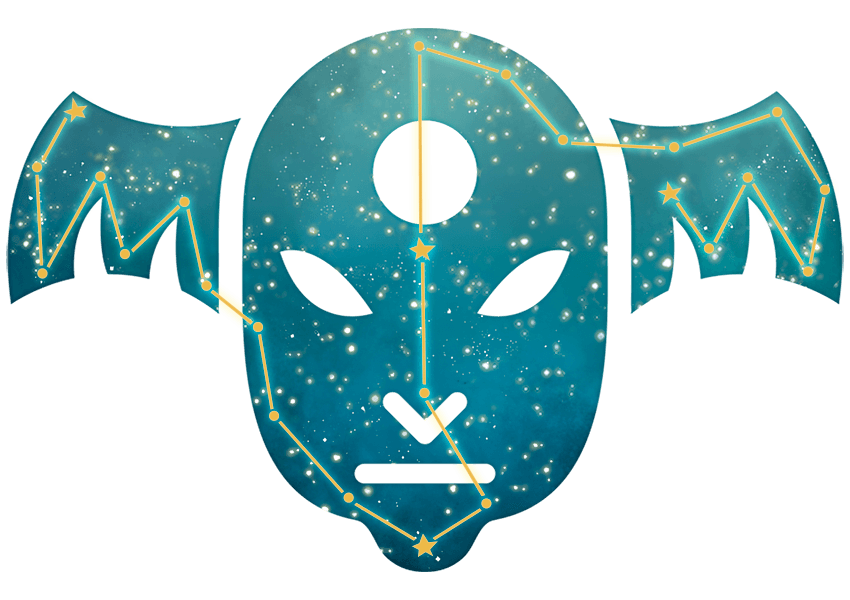
\includegraphics[width=0.47\textwidth]{02viphoger/img/10s_phenax.png}
    % \end{figure}

    \subsubsection{Worshiping Phenax}
        Every lie is an homage to Phenax.
        Because their most devout followers are criminals and gamblers, their influence is keenly felt in gambling halls and dens of thieves.
        But everyone has their own reasons to stray from the truth at times, and thus, they also find small ways to seek Phenax's favor as they go about their daily lives.

        Formal services to Phenax are conducted at night, with the most sacred rituals performed on nights of the new three moons.
        Offerings are made to attract Phenax's favor, with valuables from successful robberies, parchment filled with lies, or loaded dice being thrown into deep crags or buried at crossroads.
        Such sacrifices often vanish soon after, claimed by the god or their servants.
        Devout criminals often offer Phenax stolen goods as part of their preparations for premeditated crimes.

        % Phenax is worshiped openly in the necropoleis of Asphodel and Odunos, though the Returned who are loyal to Erebos's agent, Tymaret, refuse to worship the god they're hunting.
        % Somber ceremonies are intoned to bless the golden funeral masks the Returned wear.
\subsection*{Purphoros, God of the Forge} \label{ssec::purphoros}
    \subparagraph{Domains} Red.

    Purphoros is the god of the forge, the restless earth, and fire.
    They rule the raw creative force that infuses sapient minds.
    Purphoros is also the god of artisans, obsession, and the cycle of creation and destruction.

    As a forge radiates heat in the area around it, Purphoros's influence provides inspiration to mortals.
    They makes exquisitely crafted objects almost constantly, sometimes absentmindedly working while they holds conversations with the other gods, only to destroy the finished product and begin again.
    % Impulsive and mercurial, Purphoros is prone to bouts of either joyous productivity or frustrated anger.
    Purphoros often feels constrained by the limits of imagination, yearning to realize ideas that seem just out of reach.

    Purphoros's preferred form is that of a muscular treb gat whose coal-hued skin is mostly covered in mutable organic bronze.
    They might also appear in the form of a phoenix or a bull made of cooling lava, and for that reason, both of those creatures are associated with them.
    When angered, they might appear as an enormous mass of lava, a blazing fire, or a volcanic eruption.
    Mortals who see Purphoros in one of those forms seldom live to tell about it.

    % \begin{figure}[b]
    %     \centering
    %     
\includegraphics[width=0.47\textwidth]{02viphoger/img/10s_purphoros.png}
    % \end{figure}

    \subsubsection{Worshiping Purphoros}
        Purphoros holds dominion over everything that springs from mortal ingenuity.
        Most artisans say a small prayer to them upon beginning or completing the construction of nearly anything, from swords to fortresses to ships.

        Naturally, Purphoros is strongly associated with the forge, and nearly every smithy on Viphoger is a sort of ad hoc temple to them.
        Charms and idols of Purphoros hang from the walls in such places, intended both to inspire the artisans and protect them against accidents.
        Regardless of their professions, worshipers of Purphoros often light small fires in the god's honor, burning wooden crafts or drawings of their inventions to gain their favor.

% \pagebreak

% \begin{tikzpicture}[remember picture,overlay]
%     \node[anchor=north, yshift=0.10cm] at (current page.north) {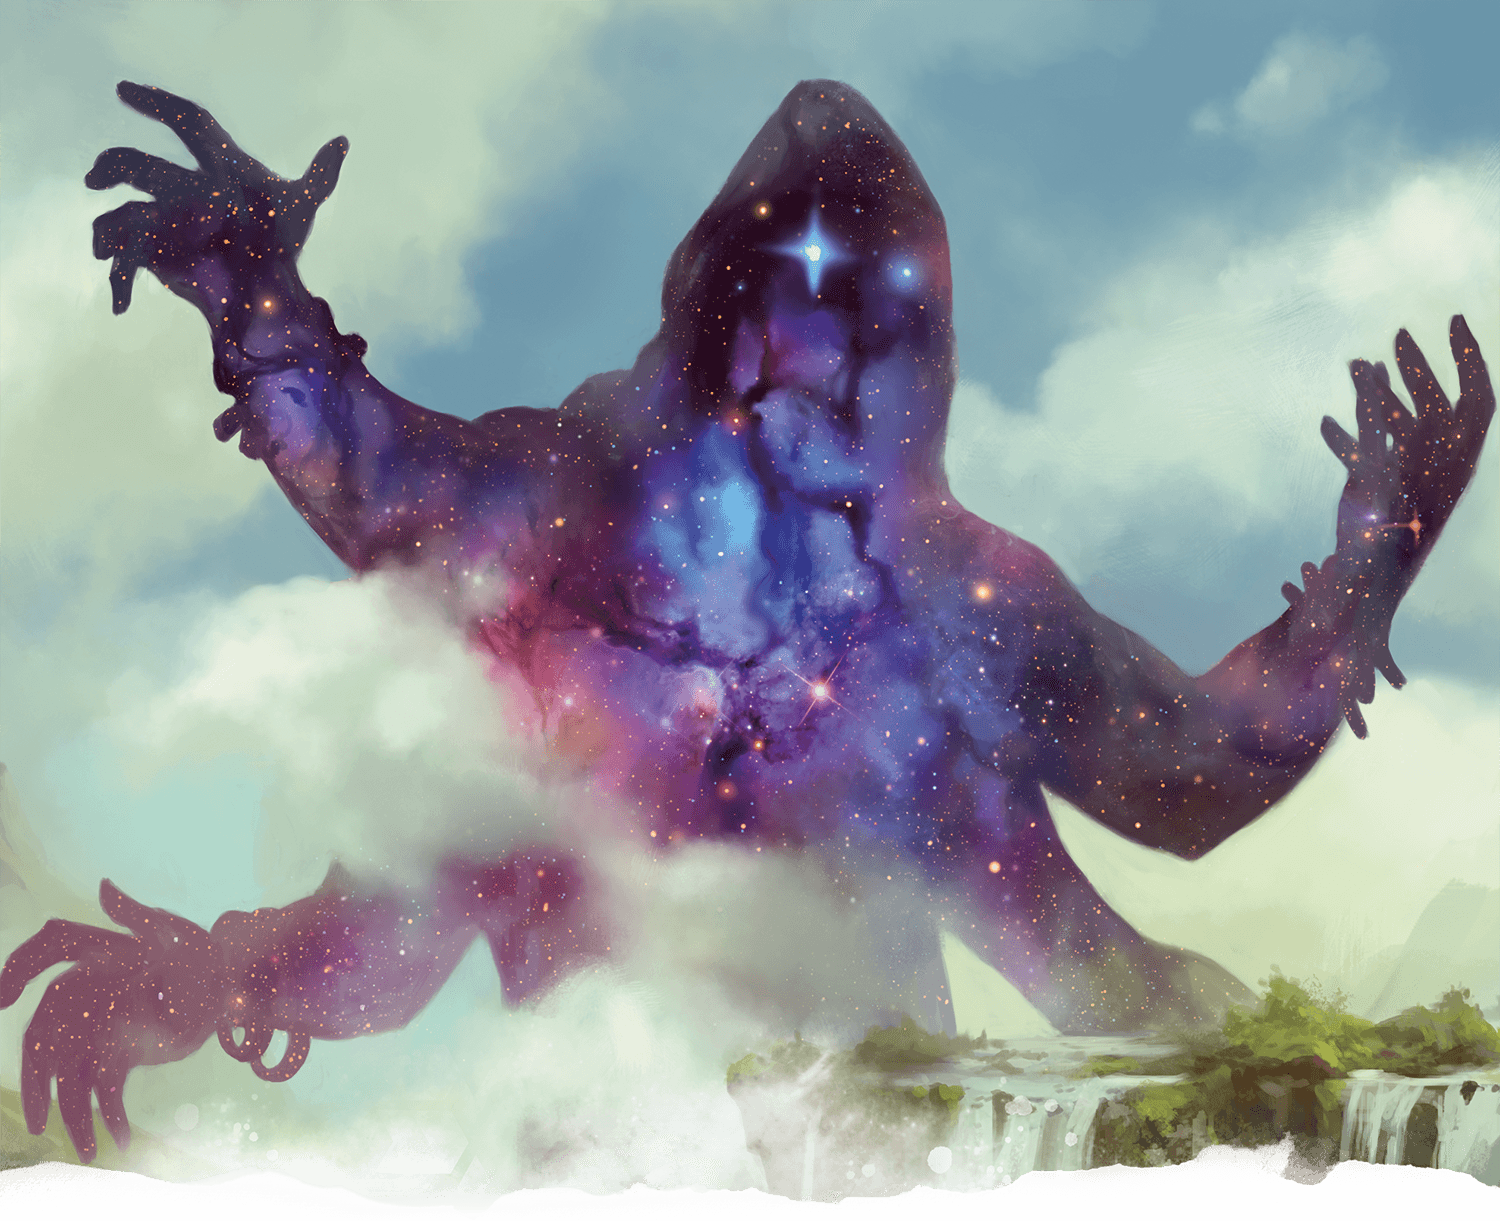
\includegraphics[width=\pdfpagewidth]{02viphoger/img/10kruphix.png}};
% \end{tikzpicture}
%
% \vspace{15.0cm}

\subsection*{Thassa, God of the Sea} \label{ssec::thassa}
    \subparagraph{Domains} Blue.

    Thassa is the god of the sea, aquatic creatures, and the unknown depths.
    She also holds sway over less tangible concepts such as ancient knowledge, long voyages, and gradual change.

    % Impassive and slow to anger, Thassa is secure in the knowledge that there are no mortals and few gods who can threaten her status.
    % Once her ire is aroused, however, it is as unstoppable as a cresting wave.
    % She often speaks in the future tense, referring to what tomorrow will bring.
    % She seldom laughs, and when she does, it is usually out of smugness rather than genuine mirth.

    Thassa usually appears to mortals in the form of a female tortle-like being with octopus-tentacle hair and a crown of crab legs.
    % She seldom adopts the same size as her followers, preferring to be seen from a distance as she towers over the ocean.
    When she moves close to the view of mortals, she takes many other forms, often shifting from one to another: a giant squid, an ocean storm, a school of sharks, a fog bank, or a crab, her favored animal.
    % She sometimes speaks out of the ocean itself, in droplets hissing across the surface of the waves.

    % \begin{figure}[b]
    %     \centering
    %     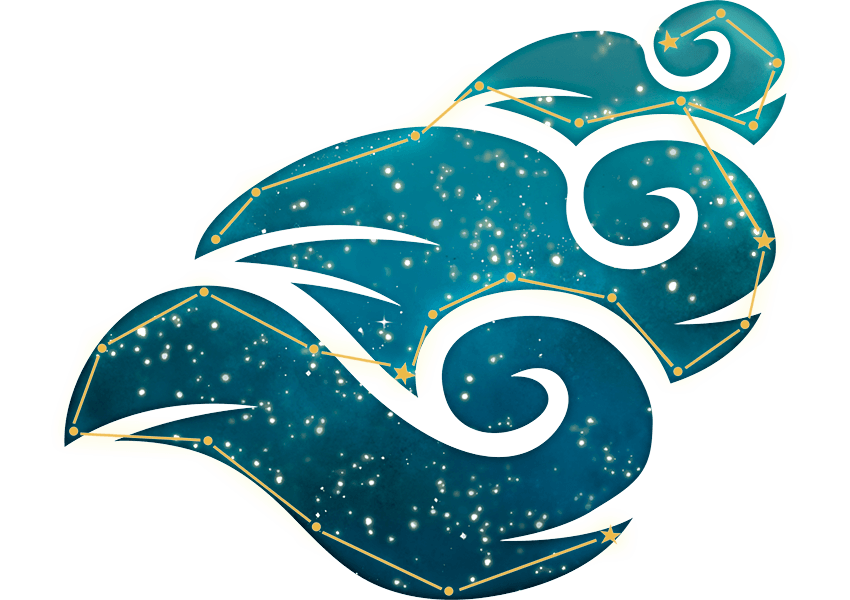
\includegraphics[width=0.47\textwidth]{02viphoger/img/10s_thassa.png}
    % \end{figure}

    \subsubsection{Worshiping Thassa}
        Most of Thassa's dedicated worshipers are tortles.% , and the vast majority of tortles are wholly devoted to Thassa.
        Tortles spend much of their lives in Thassa's realm, with their god omnipresent.
        They weave prayers to Thassa into nearly everything they do.

        Among the poleis, Thassa is worshiped by those who rely on bountiful seas for sustenance or calm waters for safety.
        Sailors, fishers, and residents of Viphoger's coasts and islands all pay her at least nominal respect and sacrifice.

        % Her center of worship on land is in the coastal polis of Mephetis, where sailors and philosophers pray to her for guidance.
        % The week-long Lyokymion festival (the Feast of the Melting Swell) marks the start of the new year by celebrating the bounty of the sea.

        % Thassa's most fervent gat worshipers offer prayers at high and low tide.
        % If possible, they do so at the water's edge.
        % At low tide they walk barefoot out onto the tidal flats, relishing the touch of Thassa's seabed.

\newpage

% !TEX root = ../main.tex
\subsection*{Piety \& Boons} \label{ssec::pietyandboons}
Being a god's champion carries no benefits in and of itself.
The gods do reward the devotion of their champions, though.
The strength of your devotion to your god is measured by your piety score.
As you increase that score, you gain blessings from your god.

Piety has nothing to do with faith or belief, except insofar as a person's thoughts and ideals drive them to action in a god's service.
Your piety score reflects the actions you have taken in your god's service --- actions that the god richly rewards.

When you choose a god to worship, your piety score related to that god is 0.
Your piety score increases by 1 when you do something to advance the god's interests or behave in accordance with the god's ideals.
The gods expect great deeds from their champions, so your piety score typically increases only when you accomplish a significant goal, make a significant sacrifice of your own self-interest, or otherwise when the DM sees fit.

The gods bestow favors on those who prove their devotion.
When your piety score crosses certain thresholds --- 3, 10, 25, and 50 --- you gain a benefit detailed in this section of your choice.
If your piety score exceeds and then falls below one of those thresholds, you lose the benefit you gained at the higher tier.

\subsubsection{Piety 3+}
    \subparagraph{Agonizing Strikes}
        You can add your Wisdom modifier to the damage of an attack.
        You can use this feature a number of times equal to your Wisdom modifier.
        You regain all expended uses of this feature when you finish a short rest.
    \subparagraph{Beast Speech}
        You can comprehend and verbally communicate with any creature with an Intelligence score of 5 or less.
    \subparagraph{Godly Influence}
        Your proficiency level in Persuasion and Deception is increased by 1.
    \subparagraph{Hero's Vigor}
        You gain 1d4 + 4 temporary hit points after you finish a short rest.
    \subparagraph{Nyx's Shield}
        While you're not wearing an armor, your AC is 12 + your Dexterity modifier.
        You can use a shield and retain this benefit.
    \subparagraph{Pact Weapon}
        During a long rest, you mark a weapon of your choice as a symbol to your god.
        That weapon is infused with your god's power, gaining a +1 bonus to attack and damage rolls for you until you finish a long rest.
    \subparagraph{Unyielding Sight}
        You can see in darkness to a distance of 24 meters.

\pagebreak

\subsubsection{Piety 10+}
    \subparagraph{A God's Gaze}
        Once per short rest, you can use an action to see through solid objects and darkness up to a range of 6 meters.
        This effect lasts for a minute.
    \subparagraph{Fagalian Cloak}
        Once per short rest, you can activate a godly aura to a radius of 1-meter around yourself as an action.
        You gain advantage on Intimidation checks while the aura is active, and all unfriendly creatures in the aura take necrotic damage equal to your Wisdom modifier (minimum of 1) at the start of their turns.
        This effect lasts for a minute or until you dismiss it as an action.
    \subparagraph{Freedom of Movement}
        You cannot be affected by difficult terrain, and your speed cannot be reduced except when you are restrained.
    \subparagraph{Godly Gift}
        You gain access to one spell with a spell point cost equal to 0.
        The spell is chosen by your DM, and pertains to your god.
    \subparagraph{Heavenly Protection}
        Once per short rest, you can negate all damage from one attack made against you as a reaction.
        You can use this ability after you know how much damage the attack would make.
    \subparagraph{Hero's Smite}
        All your successful melee attacks deal 1 force damage in addition to their normal damage.
    \subparagraph{Nyx's Veil}
        When you are in dim light or darkness, you can use two actions to become invisible.
        This invisibility remains until you take an action or reaction.

\subsubsection{Piety 25+}
    Your two boons are improved in a manner chosen by your DM.
    In addition, you can change one or both of your previously selected boons.

\subsubsection{Piety 50+}
    An ability score of your choice is increased by 2, as is your maximum for that score.
    In addition, you become a champion of your god, and they can grant you an artifact pertaining to them.

\newpage

